% chktex-file 13
% chktex-file 44
% chktex-file 24

\documentclass[../main]{subfiles}

\begin{document}

\subsection{HemeLB}\label{sec:hemelb}

Computational fluid dynamics represents a significant use case for high performance computing in many fields of engineering and science.
Of the many techniques available in this field, the lattice Boltzmann method (LBM) has gained traction in the community for its ability to be both simply deployed for parallel computation and its facility to handle complex geometric and moving boundary conditions.
The HemeLB code\footnote{\url{https://github.com/hemelb-codes}} uses the LBM to study 3D blood flow in human-scale vascular domains and has been optimised to handle the sparse geometries characteristic of these problems.
In previous work, the CPU version of the code has been shown to display strong scaling to over 300,000 cores on SuperMUC-NG (\textbf{citation}) whilst a GPU port of the code has displayed similar characteristics to over 18,000 NVIDIA V100 GPUs on Summit~\cite{zacharoudiou_development_2022}.

The current GPU ports of HemeLB have been developed using the CUDA framework.
Whilst this has been suitable for the current generations of HPC infrastructure, the imminent arrival of alternative accelerator hardware has necessitated the implementation of more platform-agnostic coding structures.
This effort porting to the OneAPI platform will be instructive as to the level of complexity of such a migration for a mature, detailed and highly performant application.

The OneAPI platform advocates the use of its DPCT conversion tool to convert the majority of an existing CUDA code to the DPC++ framework.
From a practical standpoint, it can be noted that the DevCloud environment that is offered for DPC++ development does not appear to natively contain the CUDA header files necessary for the conversion of an existing CUDA code with DPCT to take place.
As such, conversion needs to be done locally or on a cluster that contains both CUDA and OneAPI software.
Additionally, the majority of resources on the use of DPCT focus on simple, single file, examples of CUDA code.
In reality, porting a mature code will require the conversion and correction of several files to ensure a fully operational application is able to be compiled.
This is further complicated by features such as MPI communication between multiple GPUs.
For this current exercise, we have extracted a single HemeLB collision kernel to test the performance variation between a native CUDA implementation and that converted to DPC++.
The chosen kernel computes the single-relaxation time collision function used by the LBM to solve fluid flow within the simulation domain.
This is used to update the vast majority of sites at each time step and represents the bulk of computation within an iteration.

This kernel was extracted from the main HemeLB code and written into a single CUDA file with appropriate supporting structures and data to allow it to run on a single GPU.
This, highly simplified, script was converted to DPC++ with DPCT.
On our first attempt, the conversion yielded one error that needed to be corrected by hand.
Here it failed to convert a declaration of a constant memory array despite successfully converting several around the same location:

\begin{lstlisting}[language=C++,basicstyle=\small]
dpct::constant_memory<int, 1> _InvDirections_19(19); <--- Converted successfully
//__constant__ double _EQMWEIGHTS_19[19]; <--- Remained after DPCT conversion
dpct::constant_memory<double, 1> _EQMWEIGHTS_19(19); <--- Manually added
dpct::constant_memory<int, 1> _CX_19(19); <--- Converted successfully
\end{lstlisting}

For a updated version of the script, this error no longer occurred.

\subsubsection{Performance Analysis --- Profiling}\label{sec:hemelb_performance}
Following the conversion, we compared the performance of the native CUDA code and the converted code on the NVIDIA A100 GPUs available on the CSD3 cluster.
We also compared this to the Intel GPUs available on the Intel DevCloud environment.
This hardware however should not be regarded as comparable to the A100 cards and these results demonstrate the capacity for cross-platform deployment.
For this test we ran the kernel for the equivalent of 5000 iterations of a 100,000 site domain.
This was repeated 10 times to obtain a fair estimate of the runtime.

\begin{center}
	\begin{tabular}{||c c c||}
		\hline
		Hardware    & Code  & Average Runtime [s]     \\ [0.5ex]
		\hline\hline
		NVIDIA A100 & CUDA  & 0.398578 +/- 0.00020542 \\
		\hline
		NVIDIA A100 & DPC++ & 0.436205 +/- 0.00793029 \\
		\hline
		Intel P630  & DPC++ & 15.4501 +/- 0.0939887   \\ [1ex]
		\hline
	\end{tabular}
\end{center}

For this initial test case, it can be seen that on the common hardware tested here the conversion to the DPC++ framework and clang compiler has resulted in a 10\% drop in performance compared to the native CUDA code and NVIDIA compiler.

\begin{figure}[htp]
	\centering
	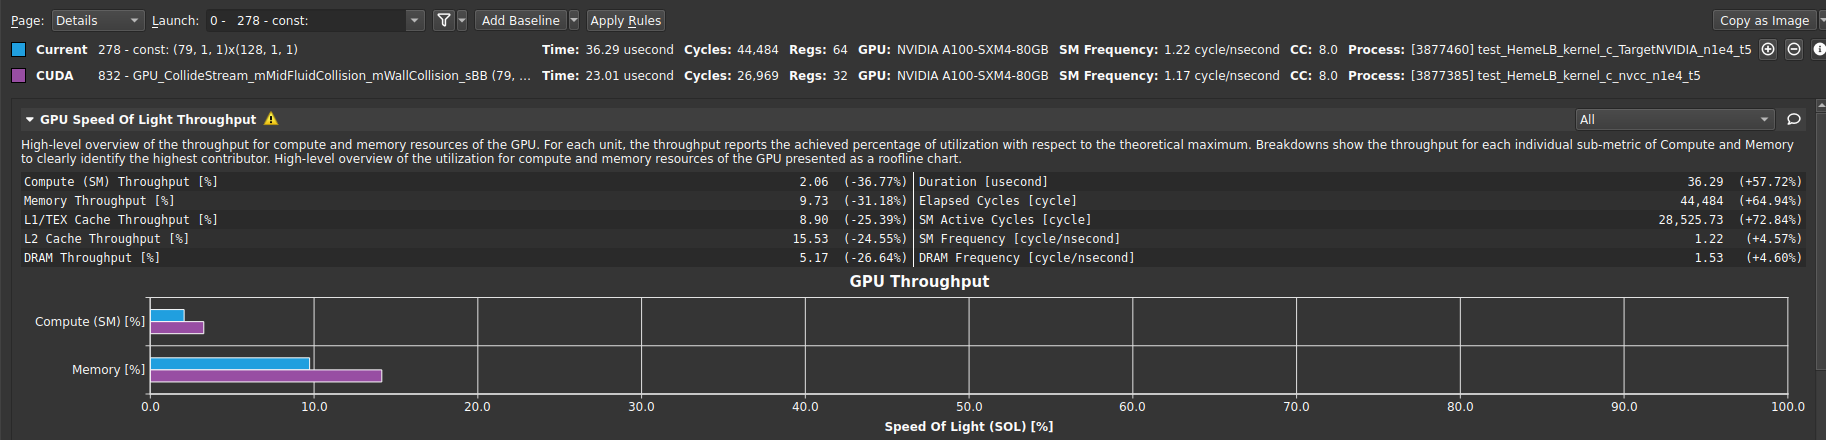
\includegraphics[clip,width=\textwidth]{Nsight_Compute_CUDA_vs_DPC++_A100_GPU.png}
	\caption{Profiling the CUDA and ported DPC++ code using NVIDIA's Nsight Compute on A100 GPU.}
	\label{fig:ncu_CUDA_Vs_DPC++_A100GPU}
\end{figure}

Profiling both versions of the code (CUDA, DPC++) was carried out using NVIDIA's performance analysis tools, Nsight Compute (see fig.~\ref{fig:ncu_CUDA_Vs_DPC++_A100GPU}) and Nsight Systems (see fig.~\ref{fig:nsys_DPC++_A100GPU}).
Nsight Compute provides detailed performance metrics at the kernel level and enables comparison of both versions, although we are not certain about the reliability of the results reported for the DPC++ code.
Nsight Compute reports a 37\% reduction of the compute throughput and a 58\% increase of the kernel's execution time compared to CUDA, while a $\sim10\%$ reduction in overall computational time was reported using either CPU timers (chrono library) or CUDA-specific timers (CUDA event API).
One issue we came across was that the profiler did not return the kernel's name for the DPC++ code.
This information was deducted from the launch statistics (gridsize and blocksize) that matched the corresponding values from profiling the native CUDA code.
The DPC++ ported function (CUDA lernel) is labelled as `const:', instead of the proper kernel's name.


Similar issues are observed with Nsight Systems.
Furthermore, the memory transactions to/from the GPU global memory are reported as memory copies to/from the Host.


\begin{figure}[htp]
	\centering
	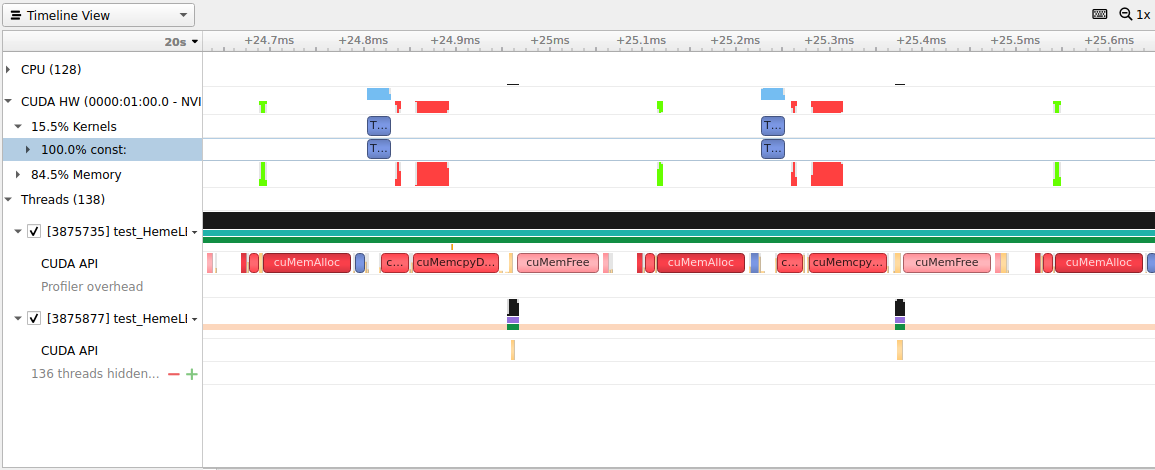
\includegraphics[clip,width=\textwidth]{profile_nsys_DPC++_A100_2steps.png}
	\caption{Profiling the ported DPC++ code using NVIDIA's Nsight Systems on A100 GPU.}
	\label{fig:nsys_DPC++_A100GPU}
\end{figure}

In this porting exercise, we have only examined HemeLB's main fluid collision kernel.
With this proof-of-concept completed, the next step would be to work through the full version of the HemeLB code to fully port it to the DPC++ format.
Being a mature code, conducting such a project port will more strongly test the capabilities to effectively port MPI-parallelised CUDA code to the OneAPI framework.

\end{document}
